\documentclass[10pt, handout]{beamer}
\usepackage{graphicx} % Required for inserting images
\usepackage{amsmath, amsthm, amssymb}
\usepackage{xcolor}

% Theme and Color Configuration
% \usetheme{Madrid}
% \usecolortheme{beaver}
% \setbeamertemplate{frame footer}{\insertshortauthor}
% \setbeamertemplate{footline}{\insertshortauthor~(\insertshortinstitute)\hfill\insertshorttitle}

\setbeamerfont{title}{size=\large}
\setbeamerfont{author}{size=\small}
\setbeamerfont{date}{size=\scriptsize}
\setbeamerfont{normal text}{size=\small}
\setbeamerfont{frametitle}{size=\large}
\setbeamerfont{block title}{size=\normalsize}
\setbeamerfont{block body}{size=\small}
\setbeamerfont{author in head/foot}{size=\tiny}


\setbeamerfont{itemize/enumerate body}{size=\small}
\setbeamerfont{itemize/enumerate subbody}{parent=itemize/enumerate body, size=\footnotesize}
\setbeamerfont{itemize/enumerate subsubbody}{parent=itemize/enumerate body, size=\scriptsize}


\usefonttheme{serif}
% \usepackage[scaled=0.95]{newpxtext}
% \usepackage{newpxmath}
\usepackage{mathpazo}

\definecolor{darkred}{rgb}{0.55, 0.0, 0.0}
\definecolor{maroon(html/css)}{rgb}{0.5, 0.0, 0.0}
\setbeamercolor{title}{fg=darkred}
\setbeamercolor{frametitle}{fg=darkred}

\setbeamercolor{theorem title}{bg=maroon(html/css)!90!white, fg=white}
\setbeamercolor{theorem body}{bg=maroon(html/css)!20!white, fg=black}
\setbeamercolor{block title}{bg=maroon(html/css)!90!white, fg=white}
\setbeamercolor{block body}{bg=maroon(html/css)!20!white, fg=black}
\setbeamercolor{author in head/foot}{fg=black!30!white}
\setbeamercolor{title in head/foot}{fg=black!30!white}

\setbeamertemplate{itemize item}[ball]
\setbeamercolor{item}{fg=darkred}
\setbeamercolor{itemize subitem}{fg=darkred}
\setbeamercolor{enumerate item}{fg=darkred}
\setbeamercolor{navigation symbols}{fg=darkred, bg=darkred!20!white}
\setbeamertemplate{footline}{%
  \begin{beamercolorbox}[ht=2.5ex,dp=2.5ex,%
    leftskip=.3cm,rightskip=.3cm plus1fil]{title in head/foot}
    \leavevmode{\usebeamerfont{title in head/foot}%
      [\insertshorttitle, \insertframenumber]}
  \end{beamercolorbox}%
}
\setbeamertemplate{navigation symbols}{}

\setbeamertemplate{blocks}[rounded][shadow=true]

\title[Causal Lab]{Causal Inference}
\subtitle{Lab9: Panel Methods -- Fixed Effects and Difference-in-Differences}
\author[Song and Park]{Xiangyu Song and Chanhyuk Park}
\institute{Washington University in St. Louis}
\date{\today}

\begin{document}

\maketitle

\begin{frame}{Topics}
  \begin{enumerate}
    \item Fixed Effects and DiD
    \vspace{0.3cm}
    \item Staggered DiD and the Problem with TWFE
    \vspace{0.3cm}
    \item Event Study Designs
    \vspace{0.3cm}
    \item Modern DiD Estimators
    \vspace{0.3cm}
    \item Factorial DiD
    \vspace{0.3cm}
    \item DiD with Continuous Treatment
    \vspace{0.3cm}

  \end{enumerate}
\end{frame}

%% ============================================================
%% PART 1: Fixed Effects and DiD
%% ============================================================

\begin{frame}{TWFE and DiD}
  \begin{itemize}
    \item The classic $2 \times 2$ DiD as a regression:
      $$
        Y_{it} = \alpha_i + \lambda_t + \tau D_{it} + \varepsilon_{it}
      $$
    \item $\alpha_i$ (unit FE) absorb level differences; $\lambda_t$ (time FE) absorb common shocks
    \item What remains is $\hat{\tau} = (\bar{Y}_{T,\text{post}} - \bar{Y}_{T,\text{pre}}) - (\bar{Y}_{C,\text{post}} - \bar{Y}_{C,\text{pre}})$
    \item With covariates: $Y_{it} = \alpha_i + \lambda_t + \tau D_{it} + X_{it}'\beta + \varepsilon_{it}$
      \begin{itemize}
        \item Only \textit{time-varying} covariates matter (time-invariant absorbed by $\alpha_i$)
        \item Avoid bad controls; cluster SEs at the unit level
      \end{itemize}
  \end{itemize}
\end{frame}

%% ============================================================
%% PART 2: Staggered DiD
%% ============================================================

\begin{frame}{Staggered DiD and the TWFE Problem (Goodman-Bacon, 2021)}
  \begin{itemize}
    \item With staggered treatment, TWFE $\hat{\tau}$ is a weighted average of all $2 \times 2$ DiD estimates:
      $\hat{\tau}^{TWFE} = \sum_{k} w_k \hat{\tau}_k$
    \item Comparisons include:
      \begin{enumerate}
        \item Early/late-treated vs.\ never-treated (good)
        \item \textbf{Early-treated vs.\ late-treated} and vice versa (problematic!)
      \end{enumerate}
    \item Already-treated units serve as ``controls'' --- but their outcomes reflect treatment!
  \end{itemize}
\end{frame}

\begin{frame}{Negative Weights in TWFE}
  \begin{itemize}
    \item Weights $w_k$ depend on group sizes and variance of $D_{it}$, \textbf{not} on what we care about --- some can be \textbf{negative}
    \item Consequence: $\hat{\tau}^{TWFE}$ can be negative even if \textit{every} unit has a positive effect
    \item Intuition: if effects grow over time, early-treated ``controls'' have rising outcomes $\to$ comparing late-treated to them biases estimates downward
    \item Takeaway: TWFE is fine \textbf{only if} treatment effects are constant across groups and over time
  \end{itemize}
\end{frame}

%% ============================================================
%% PART 3: Event Study
%% ============================================================

\begin{frame}{Event Study Designs}
  \begin{itemize}
    \item An event study lets us examine \textit{dynamic} treatment effects
    \item Define \textit{relative time}: $k = t - G_i$, where $G_i$ is the treatment adoption date for unit $i$
    \item The event study regression:
      $$
        Y_{it} = \alpha_i + \lambda_t + \sum_{k \neq -1} \tau_k \cdot \mathbf{1}[t - G_i = k] + \varepsilon_{it}
      $$
    \item $\tau_k$: treatment effect at $k$ periods relative to treatment
    \item $k = -1$ is the reference period (normalized to zero)
  \end{itemize}
\end{frame}

\begin{frame}{Interpreting the Event Study Plot}
  \begin{itemize}
    \item Pre-treatment coefficients ($k < 0$): test for parallel trends
      \begin{itemize}
        \item Should be close to zero and statistically insignificant
        \item If not $\to$ parallel trends assumption is suspect
      \end{itemize}
    \item Post-treatment coefficients ($k \geq 0$): dynamic treatment effects
      \begin{itemize}
        \item Immediate vs.\ gradual effects
        \item Fade-out or persistence
      \end{itemize}
    \item Caveat: pre-trends test has low power (absence of evidence $\neq$ evidence of absence)
  \end{itemize}
\end{frame}

\begin{frame}{Problems with TWFE Event Studies}
  \begin{itemize}
    \item The same negative-weighting problem from TWFE applies here!
    \item Sun and Abraham (2021): TWFE event study coefficients are contaminated
      \begin{itemize}
        \item Each $\hat{\tau}_k$ is a weighted average across cohorts
        \item Weights can be negative $\to$ pre-trends can look ``significant'' even when parallel trends holds
      \end{itemize}
    \item This means we can't trust either:
      \begin{enumerate}
        \item The pre-trend test (false rejections)
        \item The dynamic effect estimates (biased)
      \end{enumerate}
  \end{itemize}
\end{frame}

%% ============================================================
%% PART 4: Modern DiD Estimators
%% ============================================================

\begin{frame}{Modern Solutions}
  \begin{itemize}
    \item Several new estimators fix the TWFE problem. Key idea: \textbf{avoid using already-treated units as controls}
    \item Callaway and Sant'Anna (2021)
    \item Sun and Abraham (2021)
    \item de Chaisemartin and D'Haultf\oe uille (2020)
    \item Borusyak, Jaravel, and Spiess (2024)
    \vspace{0.2cm}
    \item All share the same core principle; differ in implementation details
  \end{itemize}
\end{frame}

%\begin{frame}{Callaway and Sant'Anna (2021)}
%  \begin{itemize}
%    \item Step 1: Estimate \textit{group-time} ATTs: $ATT(g, t)$
%      \begin{itemize}
%        \item $g$: the cohort (units first treated at time $g$)
%        \item $t$: the calendar time
%        \item Only compare cohort $g$ to not-yet-treated or never-treated units
%      \end{itemize}
%    \item Step 2: Aggregate $ATT(g,t)$ into summary parameters
%      \begin{itemize}
%        \item Overall ATT: $\overline{ATT} = \sum_{g,t} w_{g,t} \cdot ATT(g,t)$
%        \item Event study: $ATT(k) = \sum_g w_g \cdot ATT(g, g+k)$
%        \item Group-specific: $ATT(g) = \sum_t w_t \cdot ATT(g,t)$
%      \end{itemize}
%    \item R package: \texttt{did}; Stata: \texttt{csdid}
%  \end{itemize}
%\end{frame}
% 
%\begin{frame}{Sun and Abraham (2021)}
%  \begin{itemize}
%    \item Focus: fixing the event study specification
%    \item Estimate cohort-specific effects using an \textit{interaction-weighted} estimator:
%      $$
%        Y_{it} = \alpha_i + \lambda_t + \sum_{g} \sum_{k \neq -1} \delta_{g,k} \cdot \mathbf{1}[G_i = g] \cdot \mathbf{1}[t - g = k] + \varepsilon_{it}
%      $$
%    \item Then aggregate: $\hat{\tau}_k = \sum_g \hat{w}_g \hat{\delta}_{g,k}$ with proper weights
%    \item Key advantage: clean event study estimates without contamination
%    \item R: \texttt{sunab()} in \texttt{fixest}; Stata: \texttt{eventstudyinteract}
%  \end{itemize}
%\end{frame}
 
\begin{frame}{Which Estimator to Use?}
  \begin{itemize}
    \item If treatment timing varies across units $\to$ use a modern estimator
    \item Callaway \& Sant'Anna: most flexible, allows covariates, different control groups
    \item Sun \& Abraham: convenient within \texttt{fixest} framework
    \item de Chaisemartin \& D'Haultf\oe uille: allows treatment to switch on and off
    \item Practical advice:
      \begin{enumerate}
        \item Run TWFE as a baseline
        \item Run Bacon decomposition to diagnose problems
        \item Use a robust estimator as your main specification
        \item Report both for transparency
      \end{enumerate}
  \end{itemize}
\end{frame}

%% ============================================================
%% PART 5: Factorial DiD (Xu, Zhao, and Ding)
%% ============================================================

\begin{frame}{No Clean Control? Factorial DiD}
  \begin{itemize}
    \item Xu, Zhao, and Ding (forthcoming, JASA)
    \item A framework for settings where an \textbf{event affects all units}
    \item Setup: $G_i \in \{0,1\}$ (baseline factor), $Z_i \in \{0,1\}$ (universal exposure post-event)
    \item Key question: how does $G$ modify the effect of $Z$?
      \begin{itemize}
        \item E.g., does social capital ($G$) affect response to famine ($Z$)?
      \end{itemize}
    \item Challenge: all units exposed post-event $\to$ no ``pure control''
    \item Two distinct estimands:
      \begin{itemize}
        \item \textbf{Effect modification} ($\tau_{\text{em}}$): compares effects \textit{across observed subgroups}
          $\tau_{\text{em}} = \mathbb{E}[\tau_{i,Z} \mid G_i = 1] - \mathbb{E}[\tau_{i,Z} \mid G_i = 0]$
        \item \textbf{Causal moderation} ($\tau_{\text{cm}}$): causal effect of changing $G$ on the effect of $Z$
          $\tau_{\text{cm}} = \mathbb{E}[Y_i(1,1) - Y_i(1,0) - Y_i(0,1) + Y_i(0,0)]$
      \end{itemize}
  \end{itemize}
\end{frame}

\begin{frame}{Factorial DiD: Identification}
  \begin{center}
    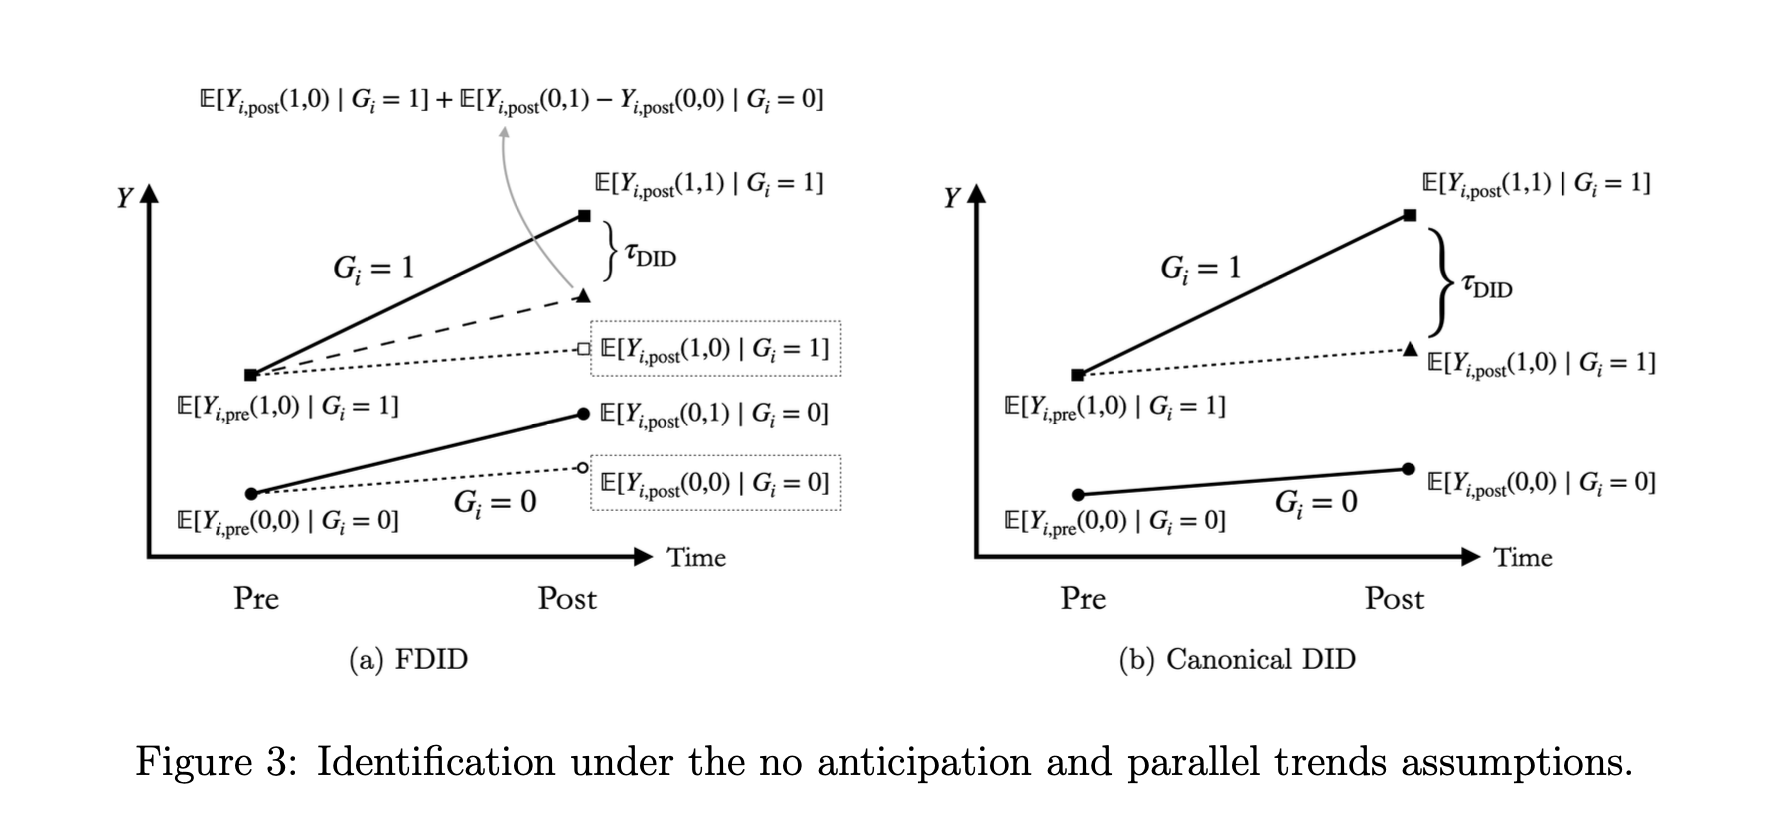
\includegraphics[width=0.75\textwidth]{fdid.png}
  \end{center}
  \vspace{-0.3cm}
  
  \begin{enumerate}
    \scriptsize
    \item \textbf{Universal exposure}: $Z_i = 1$ for all $i$ post-event
    \item \textbf{No anticipation}: $G$ does not affect outcomes before exposure
    \item \textbf{Parallel trends}: $\mathbb{E}[Y_{i,\text{post}}(0,0) - Y_{i,\text{pre}}(0,0) \mid G_i\!=\!1] = \mathbb{E}[Y_{i,\text{post}}(0,0) - Y_{i,\text{pre}}(0,0) \mid G_i\!=\!0]$
    \item \textbf{Exclusion restriction} (canonical DiD): $\mathbb{E}[Y_{i,\text{post}}(0,1) \mid G_i\!=\!0] = \mathbb{E}[Y_{i,\text{post}}(0,0) \mid G_i\!=\!0]$; $G$ has no direct post-event effect on unexposed outcomes
    \item \textbf{Factorial parallel trends} (for causal moderation): $\mathbb{E}[\Delta Y_i(g,z) \mid G_i\!=\!1] = \mathbb{E}[\Delta Y_i(g,z) \mid G_i\!=\!0]$ $\forall\, g,z$; stronger than standard PT --- enables $\tau_{\text{DID}} \to \tau_{\text{cm}}$
  \end{enumerate}
  \begin{itemize}
    \scriptsize 
    \item 2, 3, and 5 $\to \tau_{\text{em}} = \tau_{\text{cm}}$
    \item 1-3, and 5 $\to \tau_{\text{DID}} = \tau_{\text{em}} = \tau_{\text{cm}}$
  \end{itemize}
\end{frame}

\begin{frame}{Factorial DiD: Identification and Takeaways}
  \begin{itemize}
    \item Under standard parallel trends: DiD identifies \textbf{effect modification} $\tau_{\text{em}}$, \textbf{not} causal moderation
    \item To identify $\tau_{\text{cm}}$, need \textbf{factorial parallel trends} (stronger):
      $$
        \mathbb{E}[\Delta Y_i(g, z) \mid G_i = 1] = \mathbb{E}[\Delta Y_i(g, z) \mid G_i = 0] \quad \forall\, g, z
      $$
      Intuition: trends would be the same even under counterfactual $G$ values
    \item Regression: standard TWFE recovers $\tau_{\text{did}}$:
      $Y_{it} = \alpha_i + \lambda_t + \tau \cdot G_i \cdot \text{Post}_t + \varepsilon_{it}$
    \item Canonical DiD is a special case (when $G$ = treatment + exclusion restriction: $\mathbb{E} \left[ Y_{i, \text{post}}(0, 1) \mid G_i = 0 \right] = \mathbb{E} \left[ Y_{i, \text{post}}(0, 0) \mid G_i = 0 \right]$)
    \item \textbf{Takeaway}: be clear about whether you estimate effect modification or causal moderation --- they answer different questions and require different assumptions
  \end{itemize}
\end{frame}

%% ============================================================
%% PART 6: DiD with Continuous Treatment
%% ============================================================

\begin{frame}{DiD with Continuous Treatment: The Problem}
  \begin{itemize}
    \item Many settings have continuous/multi-valued treatment (e.g., minimum wage level, exposure intensity)
    \item TWFE with continuous $D_{it}$: $Y_{it} = \alpha_i + \lambda_t + \tau D_{it} + \varepsilon_{it}$
    \item Problem: $\hat{\tau}$ suffers from \textbf{negative-weighting issues} --- even worse than binary case
      \begin{itemize}
        \item TWFE implicitly compares units with different doses; no clear ``control group''
        \item Some weights are negative even under constant treatment effects (de Chaisemartin \& D'Haultf\oe uille, 2023)
      \end{itemize}
  \end{itemize}
\end{frame}

\begin{frame}{Solution: Callaway, Goodman-Bacon, and Sant'Anna (2024)}
  \begin{itemize}
    \item Define causal effects relative to a reference dose ($d = 0$):
      $ATT(d \mid d) = \mathbb{E}[Y_t(d) - Y_t(0) \mid D = d]$
    \item Summarize via the \textit{average causal response on the treated}:
      $ACRT = \mathbb{E}\!\left[\frac{\partial}{\partial d} ATT(d \mid d)\right]$
    \item Estimation: compare each dose group to untreated ($d=0$) separately, trace out the dose-response curve, then regress $\widehat{ATT}(d \mid d)$ on $d$
    \item Requires ``strong'' parallel trends: untreated potential outcomes trend the same across \textit{all} dose groups
    \item R: \texttt{did} (extended); Avoid pooling all dose levels into a single TWFE regression!
  \end{itemize}
\end{frame}

\begin{frame}{Summary: Choosing Your DiD Estimator}
  \begin{itemize}
    \item \textbf{Standard DiD / TWFE}: 2 groups, 2 periods, homogeneous effects
    \item \textbf{Callaway \& Sant'Anna / Sun \& Abraham}: staggered binary treatment, heterogeneous effects
    \item \textbf{Factorial DiD}: when events affect all units; distinguishes effect modification from causal moderation
    \item \textbf{Callaway, Goodman-Bacon, \& Sant'Anna}: continuous/multi-valued treatment
    \item \textbf{Reanalysis evidence}: modern methods usually confirm, but sometimes overturn, published findings
    \item Always think about: What comparisons is your estimator making? Are those comparisons valid?
  \end{itemize}
\end{frame}

%\begin{frame}{Practical Advice}
%  \begin{itemize}
%    \item Run the Bacon decomposition (\texttt{bacondecomp} in R/Stata) to check for problematic comparisons
%    \item Plot the event study -- both TWFE and a robust version
%    \item Be skeptical of pre-trends tests: they have low power
%    \item Think carefully about what ``not-yet-treated'' means in your setting
%    \item Report results from multiple estimators for robustness
%  \end{itemize}
%\end{frame}

\end{document}
